\chapter{Opis założeń projektu}
\label{chap:zalozenia}

Celem projektu było zaprojektowanie oraz zaimplementowanie zintegrowanego systemu informatycznego przeznaczonego do zarządzania zasobami Ochotniczej Straży Pożarnej. Stworzona aplikacja desktopowa, nazwana ,,System Zarządzania OSP'', ma na celu zastąpienie tradycyjnych, papierowych form ewidencji, oferując w zamian szybki dostęp do danych oraz ich łatwą modyfikację.

Projekt został zrealizowany jako aplikacja desktopowa, która łączy się z centralną bazą danych. Główne funkcjonalności systemu zostały podzielone na logiczne moduły, które obejmują kluczowe aspekty działalności jednostki OSP.

\begin{itemize}
    \item \textbf{System Uwierzytelniania Użytkowników:} Aplikacja posiada wbudowany ekran logowania , który weryfikuje tożsamość użytkownika na podstawie danych z bazy. System obsługuje również różne role (np. ,,admin''), co pozwala na zróżnicowanie poziomu dostępu do poszczególnych funkcji.
    \item \textbf{Moduł Zarządzania Strażakami:} Umożliwia pełne zarządzanie danymi strażaków (operacje CRUD). Przechowuje informacje takie jak dane osobowe, stopień, data wstąpienia do służby czy ważność badań lekarskich.
    \item \textbf{Moduł Zarządzania Interwencjami:} Służy do ewidencjonowania wszystkich akcji ratowniczych. Pozwala na zapisywanie szczegółów zdarzenia, takich jak data, rodzaj, miejsce, opis działań, a także lista uczestniczących w akcji strażaków i wykorzystanych pojazdów.
    \item \textbf{Moduł Zarządzania Pojazdami:} Umożliwia prowadzenie ewidencji floty pojazdów jednostki, przechowując ich oznaczenia taktyczne oraz numery rejestracyjne.
    \item \textbf{Nawigacja:} Po zalogowaniu użytkownik ma dostęp do centralnego menu, z którego może nawigować do poszczególnych modułów systemu.
\end{itemize}

Do realizacji projektu wykorzystano sprawdzone i stabilne technologie, które zapewniły odpowiednią funkcjonalność oraz wydajność aplikacji.
\begin{itemize}
    \item \textbf{Język Programowania:} Cała logika aplikacji została zaimplementowana w języku \textbf{Java}, co gwarantuje jej wieloplatformowość.
    \item \textbf{Interfejs Graficzny Użytkownika (GUI):} Interfejs został zbudowany przy użyciu biblioteki \textbf{Java Swing}, która jest standardowym narzędziem do tworzenia aplikacji okienkowych w Javie.
    \item \textbf{Baza Danych:} System opiera się na relacyjnej bazie danych \textbf{MySQL}. Nazwa schematu bazy to \texttt{szosp}.
    \item \textbf{Komunikacja z Bazą Danych:} Do połączenia aplikacji z bazą danych wykorzystano sterownik \textbf{JDBC (Java Database Connectivity)}, który jest standardowym API Javy do wykonywania zapytań SQL.
\end{itemize}



\subsection*{ Wymagania niefunkcjonalne}

Poniżej przedstawiono wymagania niefunkcjonalne dla projektu „System Zarządzania OSP”:

\begin{itemize}
    \item \textbf{Bezpieczeństwo:}
    \begin{itemize}
        \item System powinien weryfikuje tożsamość użytkownika przy pomocy loginu i hasła.
        \item Różne poziomy dostępu (np. administrator, użytkownik) ograniczają dostęp do wybranych funkcjonalności.
    \end{itemize}

    \item \textbf{Dostępność i niezawodność:}
    \begin{itemize}
        \item W przypadku problemu z połączeniem do bazy danych, użytkownik otrzymuje stosowny komunikat błędu.
    \end{itemize}

    \item \textbf{Użyteczność:}
    \begin{itemize}
        \item Interfejs graficzny jest intuicyjny i przyjazny dla użytkowników nietechnicznych.
        \item Wszystkie komunikaty i formularze są w języku polskim.
    \end{itemize}

    \item \textbf{Odporność na błędy i backup:}
    \begin{itemize}
        \item Wszystkie krytyczne operacje na danych są wykonywane w ramach transakcji.
    \end{itemize}
\end{itemize}



\chapter{Opis Struktury Projektu}
\label{chap:baza_danych}

Fundamentem aplikacji jest relacyjna baza danych o nazwie \texttt{szosp}, która została zaprojektowana w celu przechowywania i zarządzania wszystkimi informacjami dotyczącymi strażaków, pojazdów, interwencji oraz użytkowników systemu. Baza danych składa się z czterech głównych tabel oraz dwóch tabel łączących, które realizują relacje wiele-do-wielu. Schemat bazy danych został przedstawiony na diagramie encji-związków (Rys. \ref{fig:erd}).\footnote{JavaStart: JDBC – Podstawy pracy z bazą danych. \url{https://javastart.pl/baza-wiedzy/java-ee/jdbc-podstawy-pracy-z-baza-danych} [Dostęp: 14.06.2025]}

\begin{figure}[H]
	\centering
	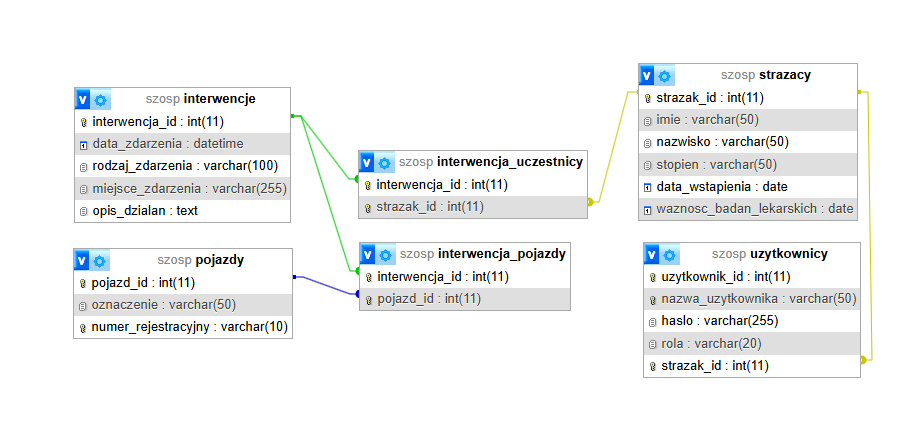
\includegraphics[width=\textwidth]{figures/BazaDanych.png}
	\caption{Diagram encji-związków (ERD) dla bazy danych \texttt{szosp}.}
	\label{fig:erd}
\end{figure}

\textbf{Tabela \texttt{strazacy}}

Tabela ta przechowuje podstawowe dane osobowe oraz służbowe każdego strażaka.

\begin{itemize}
    \item \texttt{strazak\_id}: Klucz główny, unikalny identyfikator strażaka (INT).
    \item \texttt{imie}: Imię strażaka (VARCHAR(50)).
    \item \texttt{nazwisko}: Nazwisko strażaka (VARCHAR(50)).
    \item \texttt{stopien}: Stopień służbowy (VARCHAR(50)).
    \item \texttt{data\_wstapienia}: Data wstąpienia do służby (DATE).
    \item \texttt{waznosc\_badan\_lekarskich}: Data ważności badań lekarskich (DATE).
\end{itemize}

\textbf{Tabela \texttt{uzytkownicy}}


Tabela odpowiedzialna za przechowywanie danych logowania i uprawnień użytkowników systemu.
\begin{itemize}
    \item \texttt{uzytkownik\_id}: Klucz główny, unikalny identyfikator użytkownika (INT).
    \item \texttt{nazwa\_uzytkownika}: Login użytkownika (VARCHAR(50)).
    \item \texttt{haslo}: Hasło użytkownika, przechowywane jako skrót (VARCHAR(255)).
    \item \texttt{rola}: Rola użytkownika w systemie, np. admin (VARCHAR(20)).
    \item \texttt{strazak\_id}: Klucz obcy wskazujący na powiązanego strażaka (INT).
\end{itemize}

\textbf{Tabela \texttt{pojazdy}}


Ewidencja pojazdów będących na wyposażeniu jednostki.
\begin{itemize}
    \item \texttt{pojazd\_id}: Klucz główny, unikalny identyfikator pojazdu (INT).
    \item \texttt{oznaczenie}: Oznaczenie taktyczne pojazdu (VARCHAR(50)).
    \item \texttt{numer\_rejestracyjny}: Numer rejestracyjny pojazdu (VARCHAR(10)).
\end{itemize}

\textbf{Tabela \texttt{interwencje}}


Główna tabela przechowująca informacje o przeprowadzonych interwencjach.
\begin{itemize}
    \item \texttt{interwencja\_id}: Klucz główny, unikalny identyfikator interwencji (INT).
    \item \texttt{data\_zdarzenia}: Dokładna data i czas zdarzenia (DATETIME).
    \item \texttt{rodzaj\_zdarzenia}: Kategoria zdarzenia (VARCHAR(100)).
    \item \texttt{miejsce\_zdarzenia}: Adres/lokalizacja zdarzenia (VARCHAR(255)).
    \item \texttt{opis\_dzialan}: Szczegółowy opis podjętych działań (TEXT).
\end{itemize}

\textbf{Tabele Łączące}


W celu zrealizowania relacji wiele-do-wielu, w projekcie wykorzystano dwie tabele pośredniczące.
\begin{itemize}
    \item \texttt{interwencja\_uczestnicy}: Tabela łącząca interwencje ze strażakami, którzy brali w nich udział. Składa się z dwóch kluczy obcych: \texttt{interwencja\_id} oraz \texttt{strazak\_id}.
    \item \texttt{interwencja\_pojazdy}: Tabela łącząca interwencje z pojazdami, które były do nich zadysponowane. Składa się z dwóch kluczy obcych: \texttt{interwencja\_id} oraz \texttt{pojazd\_id}.
\end{itemize}

\textbf{Relacje Między Tabelami}


Diagram ERD (Rys. \ref{fig:erd}) ilustruje kluczowe powiązania między tabelami.
\begin{itemize}
    \item \textbf{Relacja jeden-do-jednego} występuje między tabelami \texttt{strazacy} a \texttt{uzytkownicy}. Każdy strażak może mieć dokładnie jedno konto użytkownika w systemie, a każde konto jest przypisane do jednego strażaka. Relacja ta jest realizowana poprzez klucz obcy \texttt{strazak\_id} w tabeli \texttt{uzytkownicy}.
    \item \textbf{Relacja wiele-do-wielu} łączy tabelę \texttt{interwencje} z tabelą \texttt{strazacy} za pośrednictwem tabeli \texttt{interwencja\_uczestnicy}. Pozwala to na przypisanie wielu strażaków do jednej interwencji oraz na udział jednego strażaka w wielu różnych interwencjach.
    \item \textbf{Relacja wiele-do-wielu} łączy również tabelę \texttt{interwencje} z tabelą \texttt{pojazdy} za pomocą tabeli \texttt{interwencja\_pojazdy}. Dzięki temu do jednej interwencji można przypisać wiele pojazdów, a jeden pojazd może być wykorzystywany w wielu akcjach.
\end{itemize}
